\chapter{Methods}

The three models that we implement
in this thesis employ methods
for auditory processing
and trajectory generation
online and in continuous time,
meeting Sermo's criteria
outlined in Section~???.
Additionally,
we construct spiking neuron models
that implement or interact with those methods
using the Neural Engineering Framework
and Semantic Pointer Architecture.

\section{Auditory periphery models}

\subsection{Brian hears software}

\section{Dynamic movement primitives}

Dynamic movement primitives (DMPs)
are a method for planning and controlling trajectories
that requires little parameter tuning
and is stable for trajectories
with many degrees of freedom.
DMPs were originally proposed by ??? Schaal,
reformulated and refined by ??? ijspeert,
and simplified for use in spiking neural networks
by ??? dewolf.
Here, we summarize the essential aspects
of the DMP framework as described by ??? dewolf,
but invite interested readers to
the previously cited works
and ??? some more DMP cites
for further details and extensions.

DMPs use dynamical systems
with specified, stable behavior
to generate trajectories
with more complicated behavior.
The main insight in the DMP framework
is to define two separate systems,
a point attractor,
and a ``canonical system.''
The point attractor pushes
the system state to
a goal, $g$, with dynamics
\begin{equation}
  \label{dmp-pointattractor}
  \tau\ddot{y} = \alpha_y(\beta_y(g - y) - \dot{y}) + f(x, g),
\end{equation}
where $y$ is the system state,
$\dot{y}$ is the system velocity,
and $\alpha_y$ and $\beta_y$ are gain terms.
$\tau$ is a scaling term
that enables to system to operate
at different timescales,
and also appears in the definition
of the canonical system.

$f(x, g)$ is a function
of the canonical system
called the ``forcing function.''
In the discrete, one-time action case,
the canonical system
has state $x$ that evolves
with dynamics
\begin{equation}
  \label{dmp-discrete}
  \tau\dot{x} =
  \begin{cases}
    1 &\text{if } x < 1 \\
    0 &\text{if } x \ge 1,
  \end{cases}
\end{equation}
Typically the initial value of $x$
is set to 0,
so the discrete forcing function
is defined over the range $[0, 1]$.
In the rhythmic case,
the state evolves with
2D oscillator dynamics
\begin{align}
  \tau \dot{x_1} &= -2 \pi x_2 \nonumber \\
  \tau \dot{x_2} &= 2 \pi x_1.
  \label{dmp-rhythmic}
\end{align}

??? Figure 3.1 from dewolf thesis

The forcing function $f(x, g)$ is
the weighted sum
over some basis functions
$\psi_i$
(see Figure~???).
In the discrete case,
the basis functions are evaluated
for the system state $x$ directly.
In the rhythmic case,
the basis functions are evaluated
for $\frac{1}{2\pi}\tan^{-1}\left(\frac{x_2}{x_1}\right) + \frac{1}{2}$,
which maps the 2D oscillator state
to the range $[0, 1]$,
allowing the forcing function to be defined
as a function of $x$ over the range $[0, 1]$
in both cases.
The goal $g$ is used
to scale the system state $x$ depending on
the initial distance to the goal.
The final equation is
\begin{equation}
  \label{dmp-forcing-func}
  f(x, g) = \frac{\sum_{i=1}^N \psi_i w_i}{\sum_{i=1}^N \psi_i} \, x(g - y_0),
\end{equation}
where $w_i$ is the weight associated with
basis function $\psi_i$ and $y_0$
is the initial position of
the system state.

Typically, Gaussian functions
tiling the range of $x$ with some overlap
are used as the basis functions
for the forcing function
(as are used in Figure~???).
??? dewolf showed that
the response curves of spiking neurons
could be used as the
basis functions instead
(as is done for general function approximation
in the Neural Engineering Framework;
see Section~???).

\section{Neural Engineering Framework (NEF)}

The Neural Engineering Framework (NEF; ??? cite)
provides a unified method of
representing and transforming information
in spiking neural networks
such that they can implement
arbitrary dynamical systems.
The NEF is the most prominently used
tool in this thesis,
and greatly influenced the
development of the conceptual Sermo model
through the constraints and assumption
inherent in the NEF.

The NEF defines three principles that
can be used to build large-scale networks
using any spiking or non-spiking neuron model.

\subsection{Representation}
\label{sec:representation}

The representation scheme in the NEF
is based on \textit{population coding},
which was first proposed by
??? Georgoplous et al
based on experiments in monkey cortex.
Population coding is a type of distributed representation,
theorizing that an ensemble of neurons
collectively represents information.
In the original ??? Georgoplous experiment,
the ensemble of neurons coded
for the direction of a reach ??? check;
in other words,
a two-dimensional vector.
The NEF generalizes
this type of neural representation to
$n$-dimensional vector spaces,
and higher-level representations
like functions and vector fields.

The representation principle in the NEF
defines a nonlinear encoding process
and a weighted linear decoding process.
In encoding,
we aim to distribute the representation
of a vector, $\V{x}$,
by injecting current, $J$,
in a neuron model,
yielding neural activity $a(J)$.
The exact neural activity depends on
a nonlinear function, $G[\cdot]$,
which is defined by the neuron model.

In this thesis, we will primarily use
leaky integrate-and-fire (LIF) neurons.
LIF neurons are defined by the differential equation
\begin{equation*}
  \frac{dV}{dt} = - \frac{1}{RC} \left(V(t) - J(t) R\right),
\end{equation*}
where $R$ is resistance, $C$ is capacitance,
and $V(t)$ is voltage at time $t$.
When $V(t)$ reaches a threshold $V^{th}$,
the model ``spikes,''
meaning that the time of the spike,
$t_s$, is recorded,
and the voltage, $V(t)$, is reset to baseline.

In the general case,
the neural activity $a(J)$
is determined by direct simulation.
However, the LIF neuron is
simple enough that it can be
solved for directly.
\begin{equation}
  \label{eq:lif-activity-j}
  a(J) = G[J] =
  \begin{cases}
    \textstyle
    \frac{1}{\tau^{ref} - \tau^{RC} \ln \left(1 - \frac{J^{th}}{J}\right)} & \text{if } J > J^{th} \\
    0 & \text{otherwise},
  \end{cases}
\end{equation}
where $\tau^{ref}$ is the refractory time constant,
$\tau^{RC}$ is the RC time constant,
and $J^{th}$ is the current threshold
above which the neuron will spike.

The remaining question, then,
is how to relate the desired vector
$\V{x}$ to the input current
$J$ for each cell.
To do this, we first assign some
attributes to each neuron in the ensemble
that will represent $\V{x}$.
\begin{itemize}
  \item $\V{e}$ is a unit length \textit{encoder}
    that specifies the direction in vector space
    to which the neuron is sensitive.
  \item $alpha$ is a gain term that scales
    incoming signals.
  \item $J^{bias}$ is background current that
    is always present, biasing the cell
    to spike or not spike at varying input levels.
\end{itemize}
Then, the amount of current that is injected
in that neuron is
\begin{equation}
  J(\V{x}) = \alpha \V{e} \cdot \V{x} + J^{bias},
\end{equation}
where $\cdot$ is the dot product.
Since the dot product gives us
the projection of one vector on another,
it is high when the two vectors are similar;
effectively, the $\V{e} \cdot \V{x}$ term
tells us that neurons fire
more strongly when the input signal
is similar to the part of the vector space
that the neuron is sensitive to.
That similarity is then scaled by $alpha$
and biased by $J^{bias}$,
giving us the input current for each neuron.

The parameters associated with each neuron
can be chosen in several ways.
The most common way is to randomly sample
a distribution that is constrained
by knowledge of the system being modeled.
For example, if we are modeling an ensemble
of Purkinje cells, then the gains should
have the cell spike at between 1--150 Hz
for normal input signals.
If we are are modeling
an ensemble of brightness sensitive cells,
and there are usually
twice as many `on' neurons as `off' neurons,
then we would bias the
random generation of encoders appropriately.
Other times, the neuron parameters
are chosen in order to better implement
a particular function.
For example, if we are attempting to
implement a thresholding function
(e.g., $f(\V{x}) = 1 \text{if } \V{x} > 0.9$)
then using all positive encoders
and biases such that the cells
will only fire when $\V{x} > 0.9$.

In decoding, the goal is to estimate
the originally encoded vector $\V{x}$.
The NEF does this with a weighted sum
of the neural activities with a set
of decoding weights, $\V{d}$.
I.e.,
\begin{equation}
  \label{vec}
  \V{\hat{x}} = \sum_{i=0}^n \V{d}_i a_i,
\end{equation}
where $\V{\hat{x}}$ is the
decoded estimate of the encoded vector $\V{x}$,
$\V{d}_i$ is the decoding weight for neuron $i$,
and $a_i$ is the activity of neuron $i$.

To determine the decoding weights $\V{d}$
we minimize the reconstruction error
$\V{x} - \V{\hat{x}}$
by setting up the relation
\begin{equation*}
  \V{Ad} = \V{X},
\end{equation*}
where $\V{X}$ is a set of sample points
in the vector space,
and $A$ is a matrix with the activities
of all neurons for all neurons;
i.e.,
\begin{equation*}
  \label{A}
  \V{A} =
  \begin{bmatrix}
    a_0(X_0) & a_1(X_0) & \dots  & a_n(X_0) \\
    a_0(X_1) & a_1(X_1) & \dots  & a_n(X_1) \\
    \vdots & \vdots & \ddots & \vdots \\
    a_0(X_m) & a_1(X_m) & \dots  & a_n(X_m).
  \end{bmatrix}
\end{equation*}
This equation is in the form
of a linear least squares problem,
which can be solved with standard methods
??? cite lawson and hanson 1974.
See Figure~??? for an illustration
of how the decoding vectors
result in an estimate of the encoded vector.

% \begin{figure}[ht!]
%   \centering
%   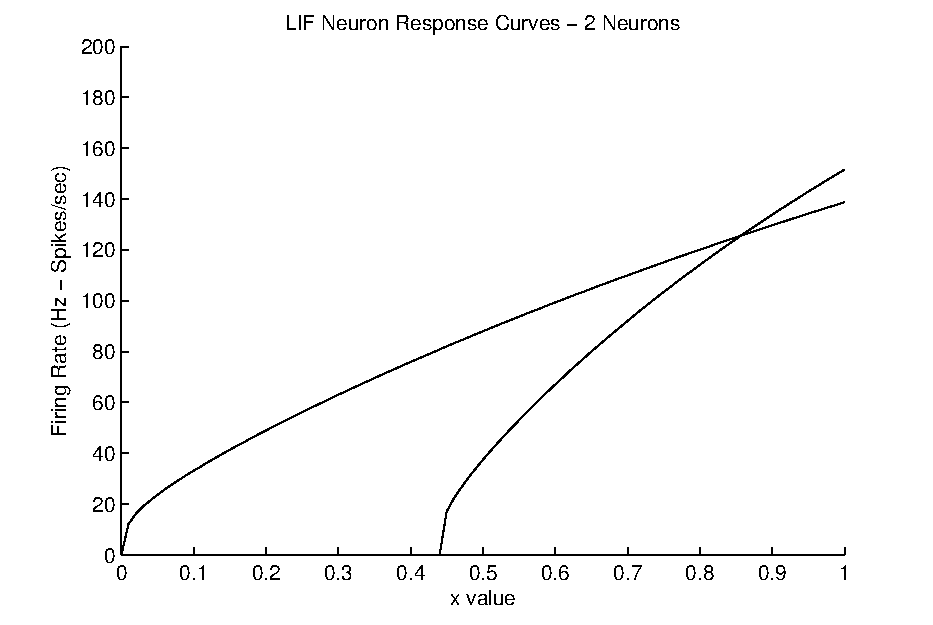
\includegraphics[width=0.45\columnwidth]{lif_est_resp_2}
%   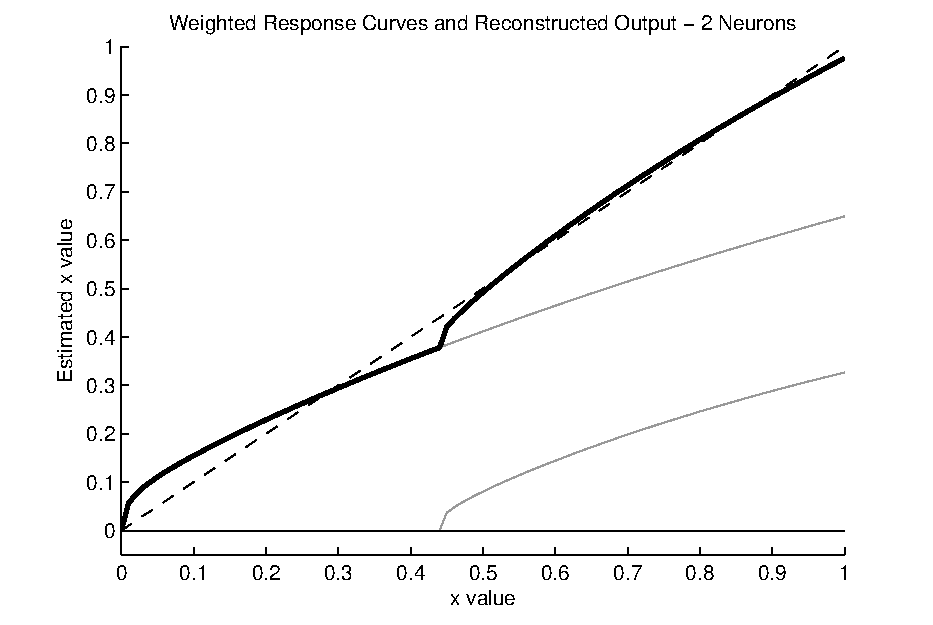
\includegraphics[width=0.45\columnwidth]{lif_est_out_2} \\
%   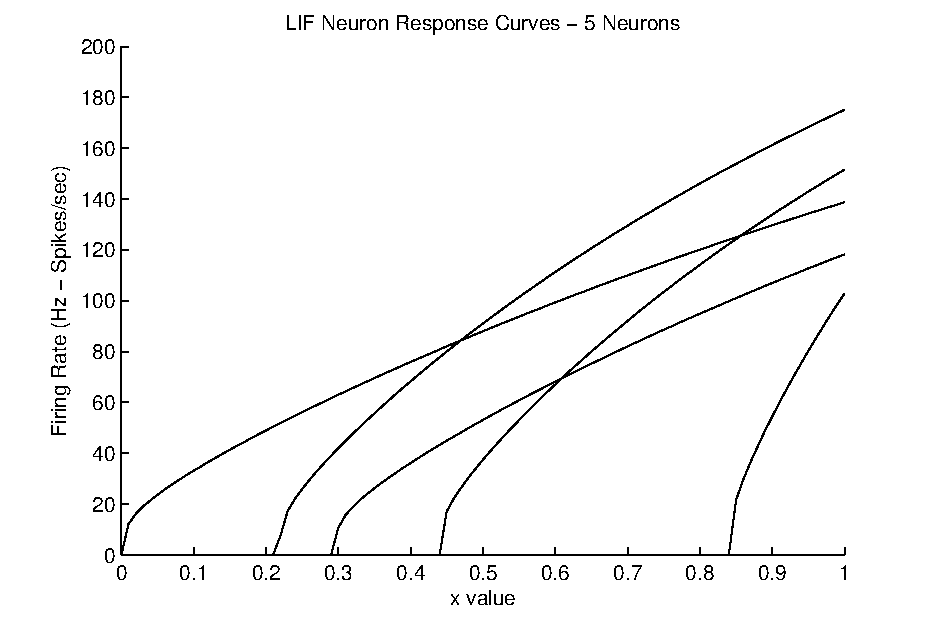
\includegraphics[width=0.45\columnwidth]{lif_est_resp_5}
%   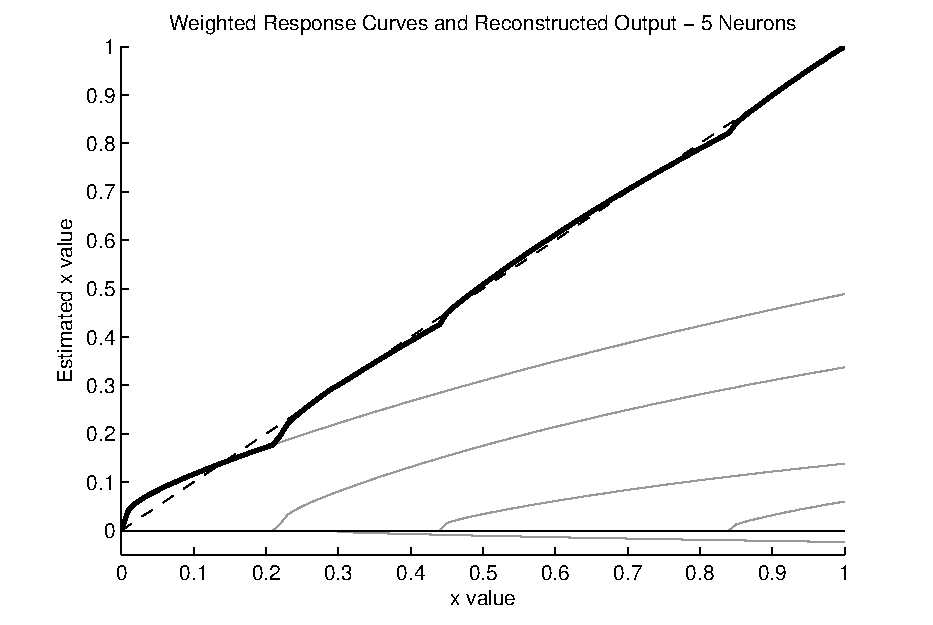
\includegraphics[width=0.45\columnwidth]{lif_est_out_5} \\
%   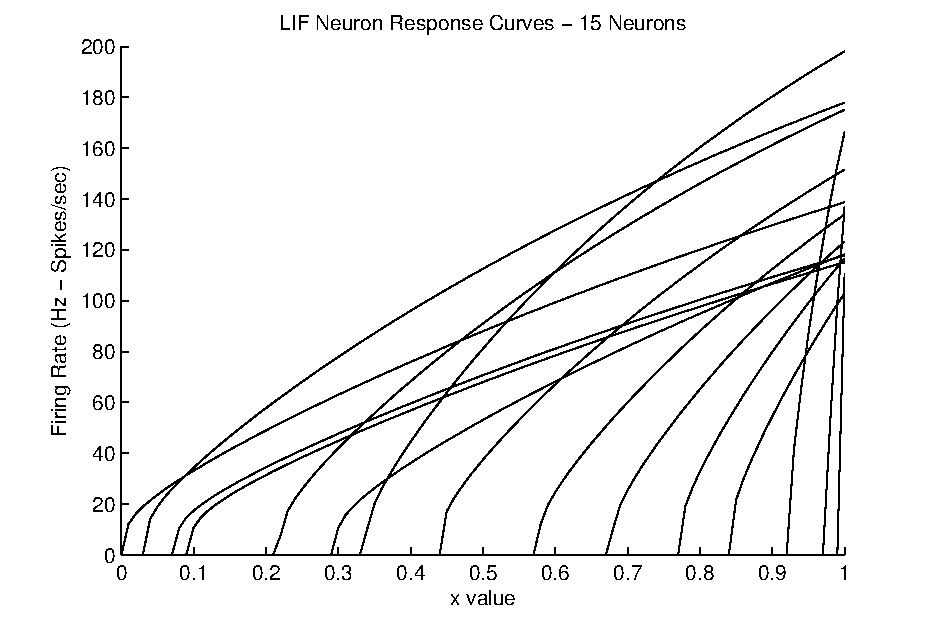
\includegraphics[width=0.45\columnwidth]{lif_est_resp_15}
%   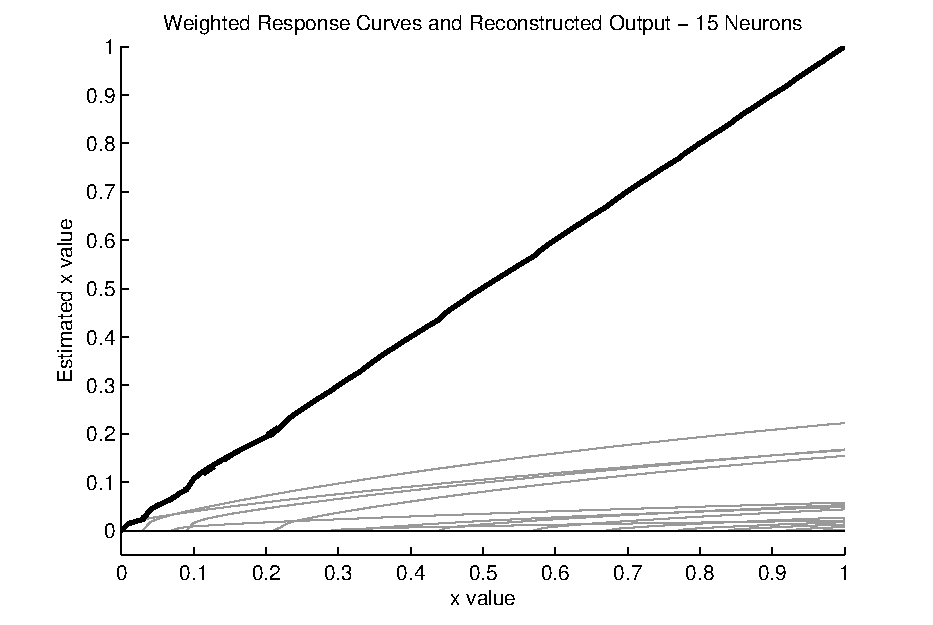
\includegraphics[width=0.45\columnwidth]{lif_est_out_15}
%   \caption{Illustration showing how the tuning curves of a population of LIF
%     neurons can be linearly combined to estimate an input signal, $x$. From
%     \cite{Choo2010}.}
%   \label{fig:dec-scalar}
% \end{figure}

For neurons with instantaneous rate equations,
like the LIF neuron (see Equation~??? ref),
the description to this point
is sufficient to encode and decode information.
However, to deal with spiking neuron models,
we must explicitly consider time,
which to this point has been an implicit
part of all of the equations.
We model neural spikes as
Dirac $\delta$ functions,
and define the time-varying
neural activity as
\begin{equation}
  \label{a(t)}
  a(t) = \sum_s \delta(t - t_s) * h(t) = \sum_s h(t - t_s),
\end{equation}
where $s$ is the set of spike times,
$*$ is the convolution operator,
and $h(\cdot)$ is a filter designed to
model the change in a neuron's current
as a result of an incoming spike
of neurotransmitter.\footnote{
  Equation~\eqref{a(t)} is also how we determine
  the steady state activity of each neuron in
  equation~\eqref{A} for neuron models
  that do not have an analytical
  instantaneous rate equation.}
Typically, we emulate post-synaptic current curves
recorded empirically by using a decaying exponential;
i.e.,
\begin{equation}
  h(t) = e^{-t / \tau^{PSC}},
\end{equation}
where $\tau^{PSC}$ is the time constant
of the exponential curve decay,
designed to match
a recorded post synaptic current (PSC) curve.

Putting these equations together,
we get the final expression for
the decoded estimate of the input $\V{x}$
using spiking neuron models,
\begin{equation}
  \label{dec-time}
  \V{\hat{x}}(t) = \sum_{i=0}^n \V{d}_i \sum_{s_i} h(t-t_{s_i}).
\end{equation}
See Figure~??? for an illustration of
the decoding process.

% \scalefigonesumm{temporal-dec}{0.8}{Decoding a time-varying
%   scalar signal using a filtered spike train.}
%   {Example of decoding a time-varying
%   scalar signal using a filtered spike train. For each spike, the
%   filter $h(t)$ is pasted in, weighted by the decoding weight
%   (1 or -1 in this case). Recreated from \cite{Eliasmith2011}.}

\subsection{Transformation}

In the representation principle,
we treated neurons as though
it were possible to directly inject current in them.
While direct current injections
can make sense for modeling
sensory systems,
the majority of neurons
receive their input from other neurons.
In the transformation principle,
the NEF defines an alternately weighted
linear decoding
that can transmit functions
of the vector represented
by one ensemble to another ensemble
through a connection weight matrix.

Given some neuron $j$
in an ensemble downstream
of an ensemble with neurons indexed by $i$,
the input current to neuron $j$ is
\begin{equation}
  \label{Jin}
  J_j = \sum_{i=0}^n \omega_{ij} a_i + J_j^{bias},
\end{equation}
where $omega_{ij}$ is the strength of the connection
between neurons $i$ and $j$.

Consider the case in which we want
an ensemble to represent
the same vector as the ensemble
providing it input;
i.e., we want to implement the function
$\V{y} = f(\V{x}) = \V{x}$.
Equation~\eqref{...} tells us how
we can approximate $\V{x}$, so let us
substitute that approximation
into equation~\eqref{...}.
\begin{align} \label{eq:jin-xhat}
  J_j &= \alpha_j \V{e}_j \cdot \V{\hat{x}} + J_j^{bias} \nonumber \\
      &= \alpha_j \V{e}_j \cdot \sum_{i=0}^n \V{d}_i a_i + J_j^{bias} \nonumber \\
      &= \sum_{i=0}^n \alpha_j \V{e}_j \cdot \V{d}_i a_i + J_j^{bias}
\end{align}

Setting \eqref{...} equal to \eqref{...},
we can rearrange terms to
obtain an equation for $\omega_{ij}$.
\begin{align} \label{eq:omega}
  \sum_{i=0}^n \omega_{ij} a_i + J_j^{bias} &= \sum_{i=0}^n \alpha_j \V{e}_j \cdot \V{d}_i a_i + J_j^{bias} \nonumber \\
  \omega_{ij} &= \alpha_j \V{e}_j \cdot \V{d}_i
\end{align}

Since the decoding process is linear,
we can implement any linear function
by introducing a matrix $L_{ji}$
that performs a different combination
of the downstream ensemble's encoders, $\V{e_j}$,
and the upstream ensemble's decoders, $\V{d_i}$.
\begin{equation}
  \omega_{ij} &= \alpha_j \V{e}_j \V{C}_{ji} \V{d}_i
\end{equation}

Since the decoding process is
a weighted summation,
we can compute the sum of
vectors of the same length
by representing those vectors
with separate ensembles
and making a connection
from each ensemble to the downstream ensemble.
\begin{align}
  \label{eq:nef-sum}
  J_j &= J_j^{\V{x}} + J_j^{\V{y}} + J_j^{bias} \nonumber \\
      &= \sum_i \omega_{ij}^{\V{x}}a_i^{\V{x}} + \sum_i \omega_{ij}^{\V{y}}a_i^{\V{y}} + J_j^{bias} \nonumber \\
  \omega_{ij}^{\V{x}} &= \alpha_j \V{e}_j \V{C}^{\V{x}}_{ji} \V{d}_i^{\V{x}} \text{ and }
  \omega_{ij}^{\V{y}} = \alpha_j \V{e}_j \V{C}^{\V{y}}_{ji} \V{d}_i^{\V{y}},
\end{align}
and so on for any number of input ensembles.

Nonlinear transformations
of some vector $\V{x}$ can be implemented
by computing a new set of decoding weights,
$\V{d}^{f(\V{x})$,
which minimizes the reconstruction error
between the estimate $\V{\hat{x}}$
and the result of applying the function,
$f(\V{x})$. I.e., equations~\eqref{...} and \eqref{...} become
\begin{align*}
  \V{A}^{f(\V{x})}d^{f(\V{x})} &= f(\V{X}) \\
  \V{A}^{f(\V{x})} &=
  \begin{bmatrix}
    a_0(f(X_0)) & a_1(f(X_0)) & \dots  & a_n(f(X_0)) \\
    a_0(f(X_1)) & a_1(f(X_1)) & \dots  & a_n(f(X_1)) \\
    \vdots & \vdots & \ddots & \vdots \\
    a_0(f(X_m)) & a_1(f(X_m)) & \dots  & a_n(f(X_m)),
  \end{bmatrix}
\end{align*}
and the remaining equations only change
in the set of decoding weights used.
See Figure~??? for an illustration
of decoding a nonlinear function.

% \begin{figure}[ht!]
%   \centering
%   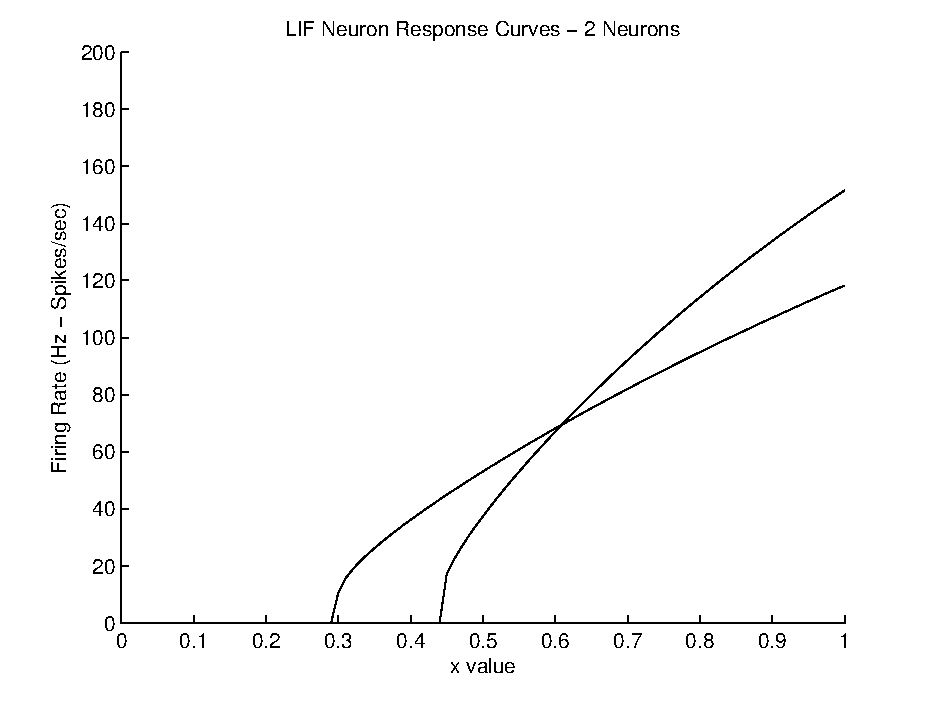
\includegraphics[width=0.45\columnwidth]{lif_func_resp_2}
%   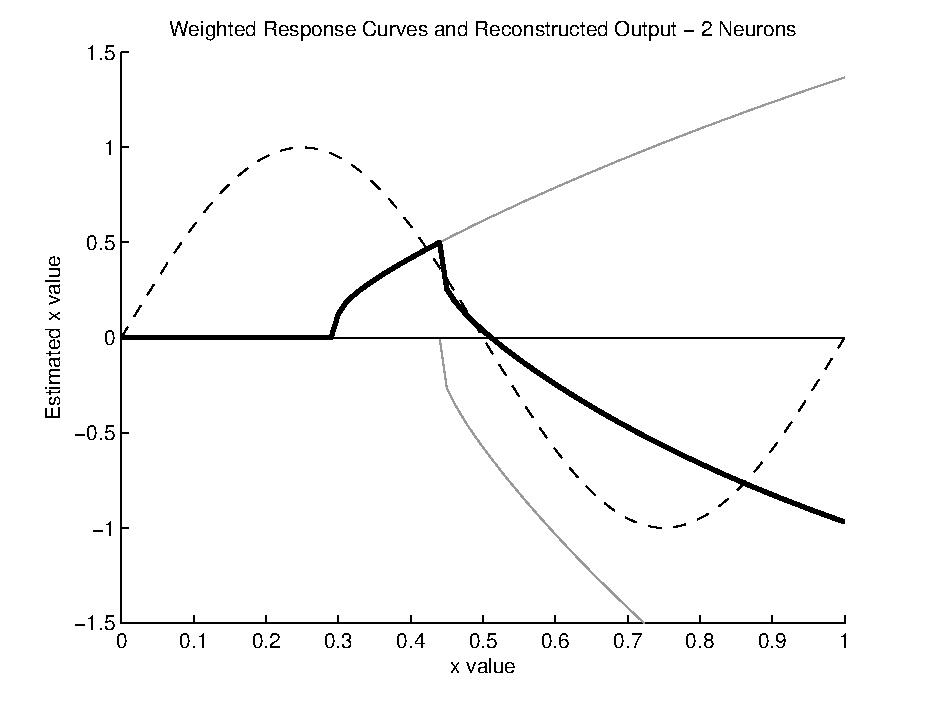
\includegraphics[width=0.45\columnwidth]{lif_func_out_2} \\
%   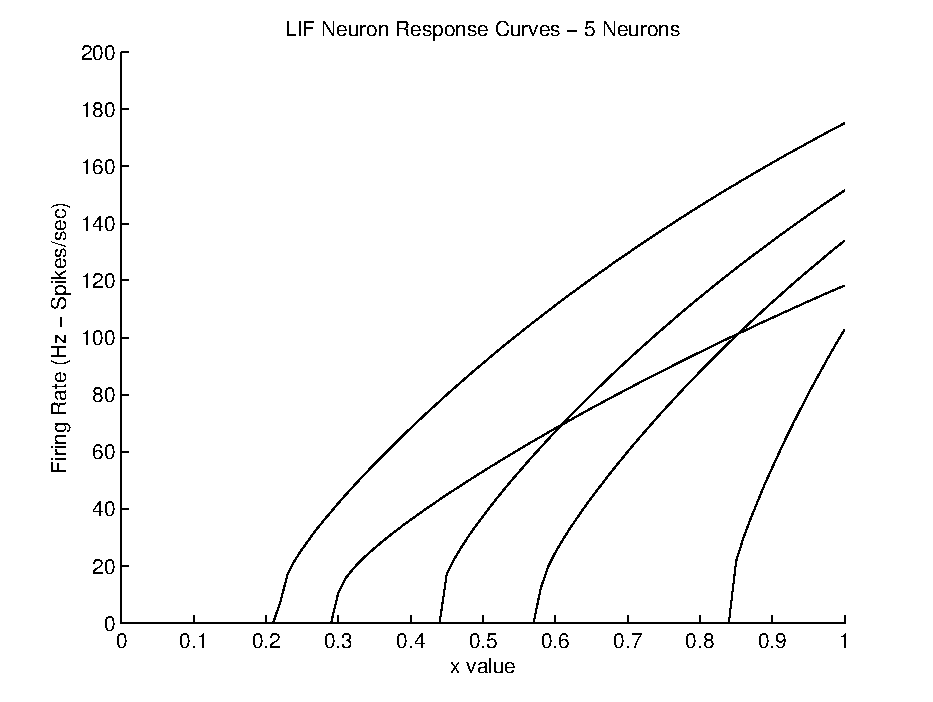
\includegraphics[width=0.45\columnwidth]{lif_func_resp_5}
%   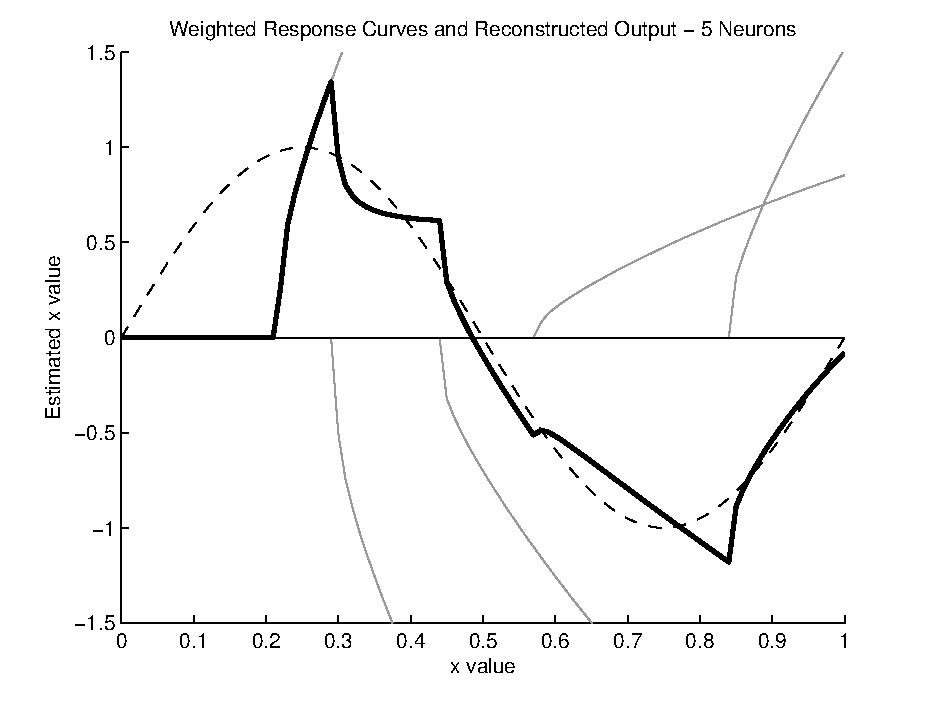
\includegraphics[width=0.45\columnwidth]{lif_func_out_5} \\
%   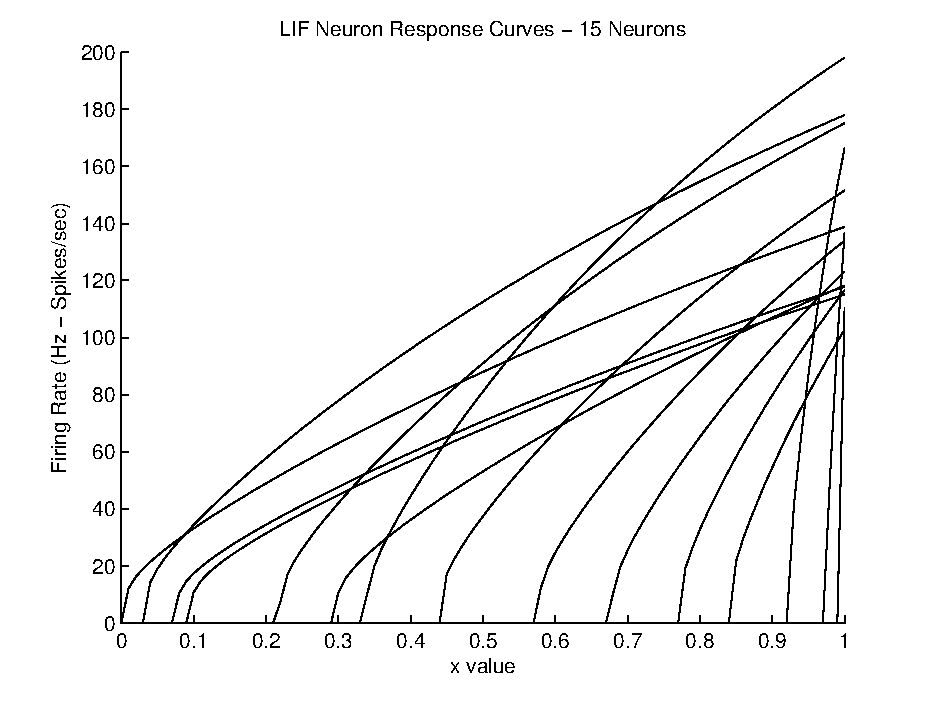
\includegraphics[width=0.45\columnwidth]{lif_func_resp_15}
%   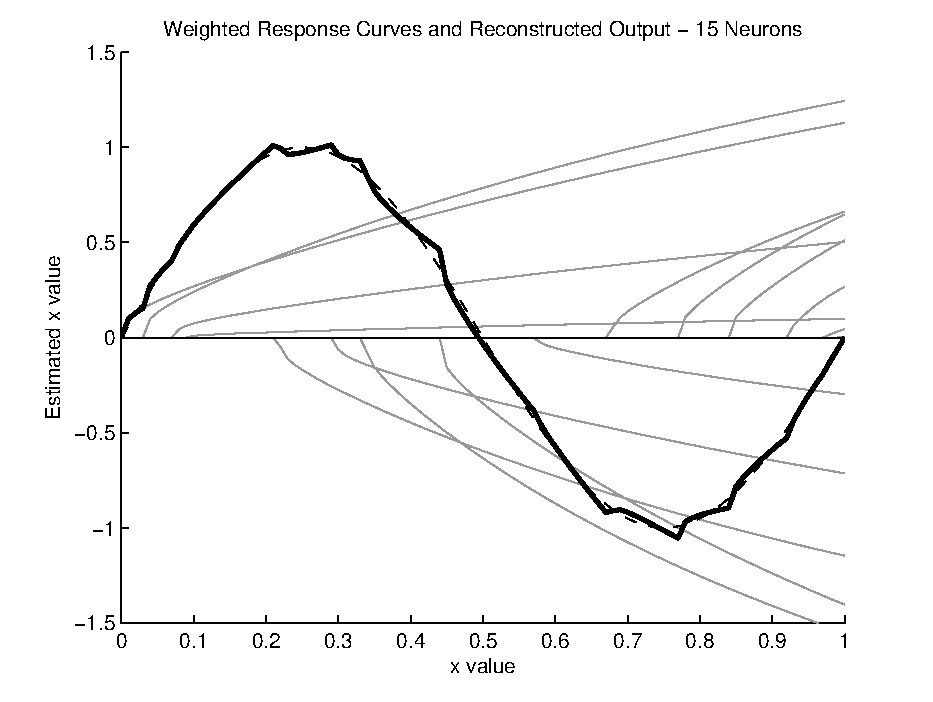
\includegraphics[width=0.45\columnwidth]{lif_func_out_15}
%   \caption{Illustration showing how the tuning curves of a population of LIF
%     neurons can be linearly combined to estimate a nonlinear function, in this
%     case $\sin(2\pi x)$. From \cite{Choo2010}.}
%   \label{fig:dec-func}
% \end{figure}

Note that this method
of computing nonlinear transformations
requires that all of the vectors
participating in the transformation
must be represented by a single ensemble.
Therefore, in order to compute
a function $f(\V{x_1}, \V{x_2})$,
a new ensemble must be created
that will represent
a vector in a space that is the concatenation
of the spaces in which $\V{x_1}$
and $\V{x_2}$ reside.

\subsection{Dynamics}

Dynamical systems have been used effectively
for control problems in several domains.
As animals are successful controllers
of cognitive and motor actions,
implementing dynamical systems
with spiking neurons seems a natural fit.
In the NEF, dynamics are implemented
by interpreting the vector
represented by some ensemble as
the state of a dynamical system,
which can implement differential equations
through recurrent connections.
No additional techniques are required
to compute recurrent connections;
the transformation principle
is used as previously described.
The dynamics principle
is instead a type of network architecture
(see Figure~???) that can
implement differential equations
as are descried in dynamical systems
and control theory.

% ??? fig 6.5 from dewolf, or htbab 2.12

The architecture depicted in Figure~???
implements a linear control system,
and can be expressed as
\begin{equation}
  \V{\dot{x}}(t) = \V{Ax}(t) + \V{Bu}(t),
\end{equation}
where $\V{A}$ is the dynamics matrix
and $\V{B}$ is the input matrix.
Normally, transforming this equation
into Laplace space results
results in dynamics scaled by
the filter $H(s) = \frac{1}{s}$.
However, the actual dynamics of the system
are based on the synaptic dynamics,
$h(t)$ from equation~\eqref{...}.
The Laplace transform of $h(t)$ is
$H'(s) = \frac{1}{1 + s\tau}$.
By accounting for the difference
between these two filters
(see ??? NEF book or htbab
for a full derivation),
we get
\begin{align}
  \V{A'} &= \tau \V{A} + \V{I} \\
  \V{B'} &= \tau \V{B},
\end{align}
where $\V{I}$ is the identity matrix.

Equations~\eqref{...} and \eqref{...}
allow us to implement any linear dynamical system
in spiking neural networks
by setting up the recurrent connection
from the ensemble representing the system state
to compute the linear transform $\tau \V{A} + \V{I}$,
and setting the transform on the connection
from the input ensemble
to the system state ensemble
to have weight $\tau \V{B}$.

Nonlinear dynamical systems can also be implemented
with a similar approach;
in essence, all that is required is to
recognize that the synaptic filter $h(t)$
introduces an exponential ``forgetting''
of the system state
which must be accounted for by scaling
connections with the time constant $\tau$
(see ??? something for more details).

\section{Semantic Pointer Architecture (SPA)}

\section{Nengo software}

% mention that Nengo takes care of a lot of annoying details.
% for example, instead of manually specifying the gain and bias,
% we specify the desired radius, x-intercepts, and maximum firing rates
% for the ensemble; Nengo figures out the gain and bias.

\subsection{Integrating Brian in Nengo}
